\documentclass[12pt, letterpaper]{memoir}
\usepackage{ExamStyle}

\begin{document}
	\pagestyle{empty}
	\begin{center}
		{\Huge Rowley CHEM 1220 Midterm 4}
	\end{center}
	
	{\large Formulas}
	
	\begin{minipage}{0.5\linewidth}
		$S=k_B\ln W$
		
	
	\end{minipage}
	\begin{minipage}{0.5\linewidth}
		$\displaystyle\Delta S^{\circ}_{rxn} = \sum\limits_{i, products} \nu_iS_i^{\circ} - \sum_{j, reactants} \nu_jS_j^{\circ}$
	\end{minipage}
	
	\vspace{2em}

	{\large Constants}
	
	$R=8.314 \dfrac{J}{mol~K}$
	
	$R=0.08206 \dfrac{L~atm}{mol~K}$
	
	$k_B=1.380649 \times 10^{-23} \dfrac{J}{K}$
	
	$N_A=6.022\times10^{23}mol^{-1}$

	
    \newgeometry{top=1mm, bottom=1mm, left=1mm, right=1mm}


\hspace{6em}	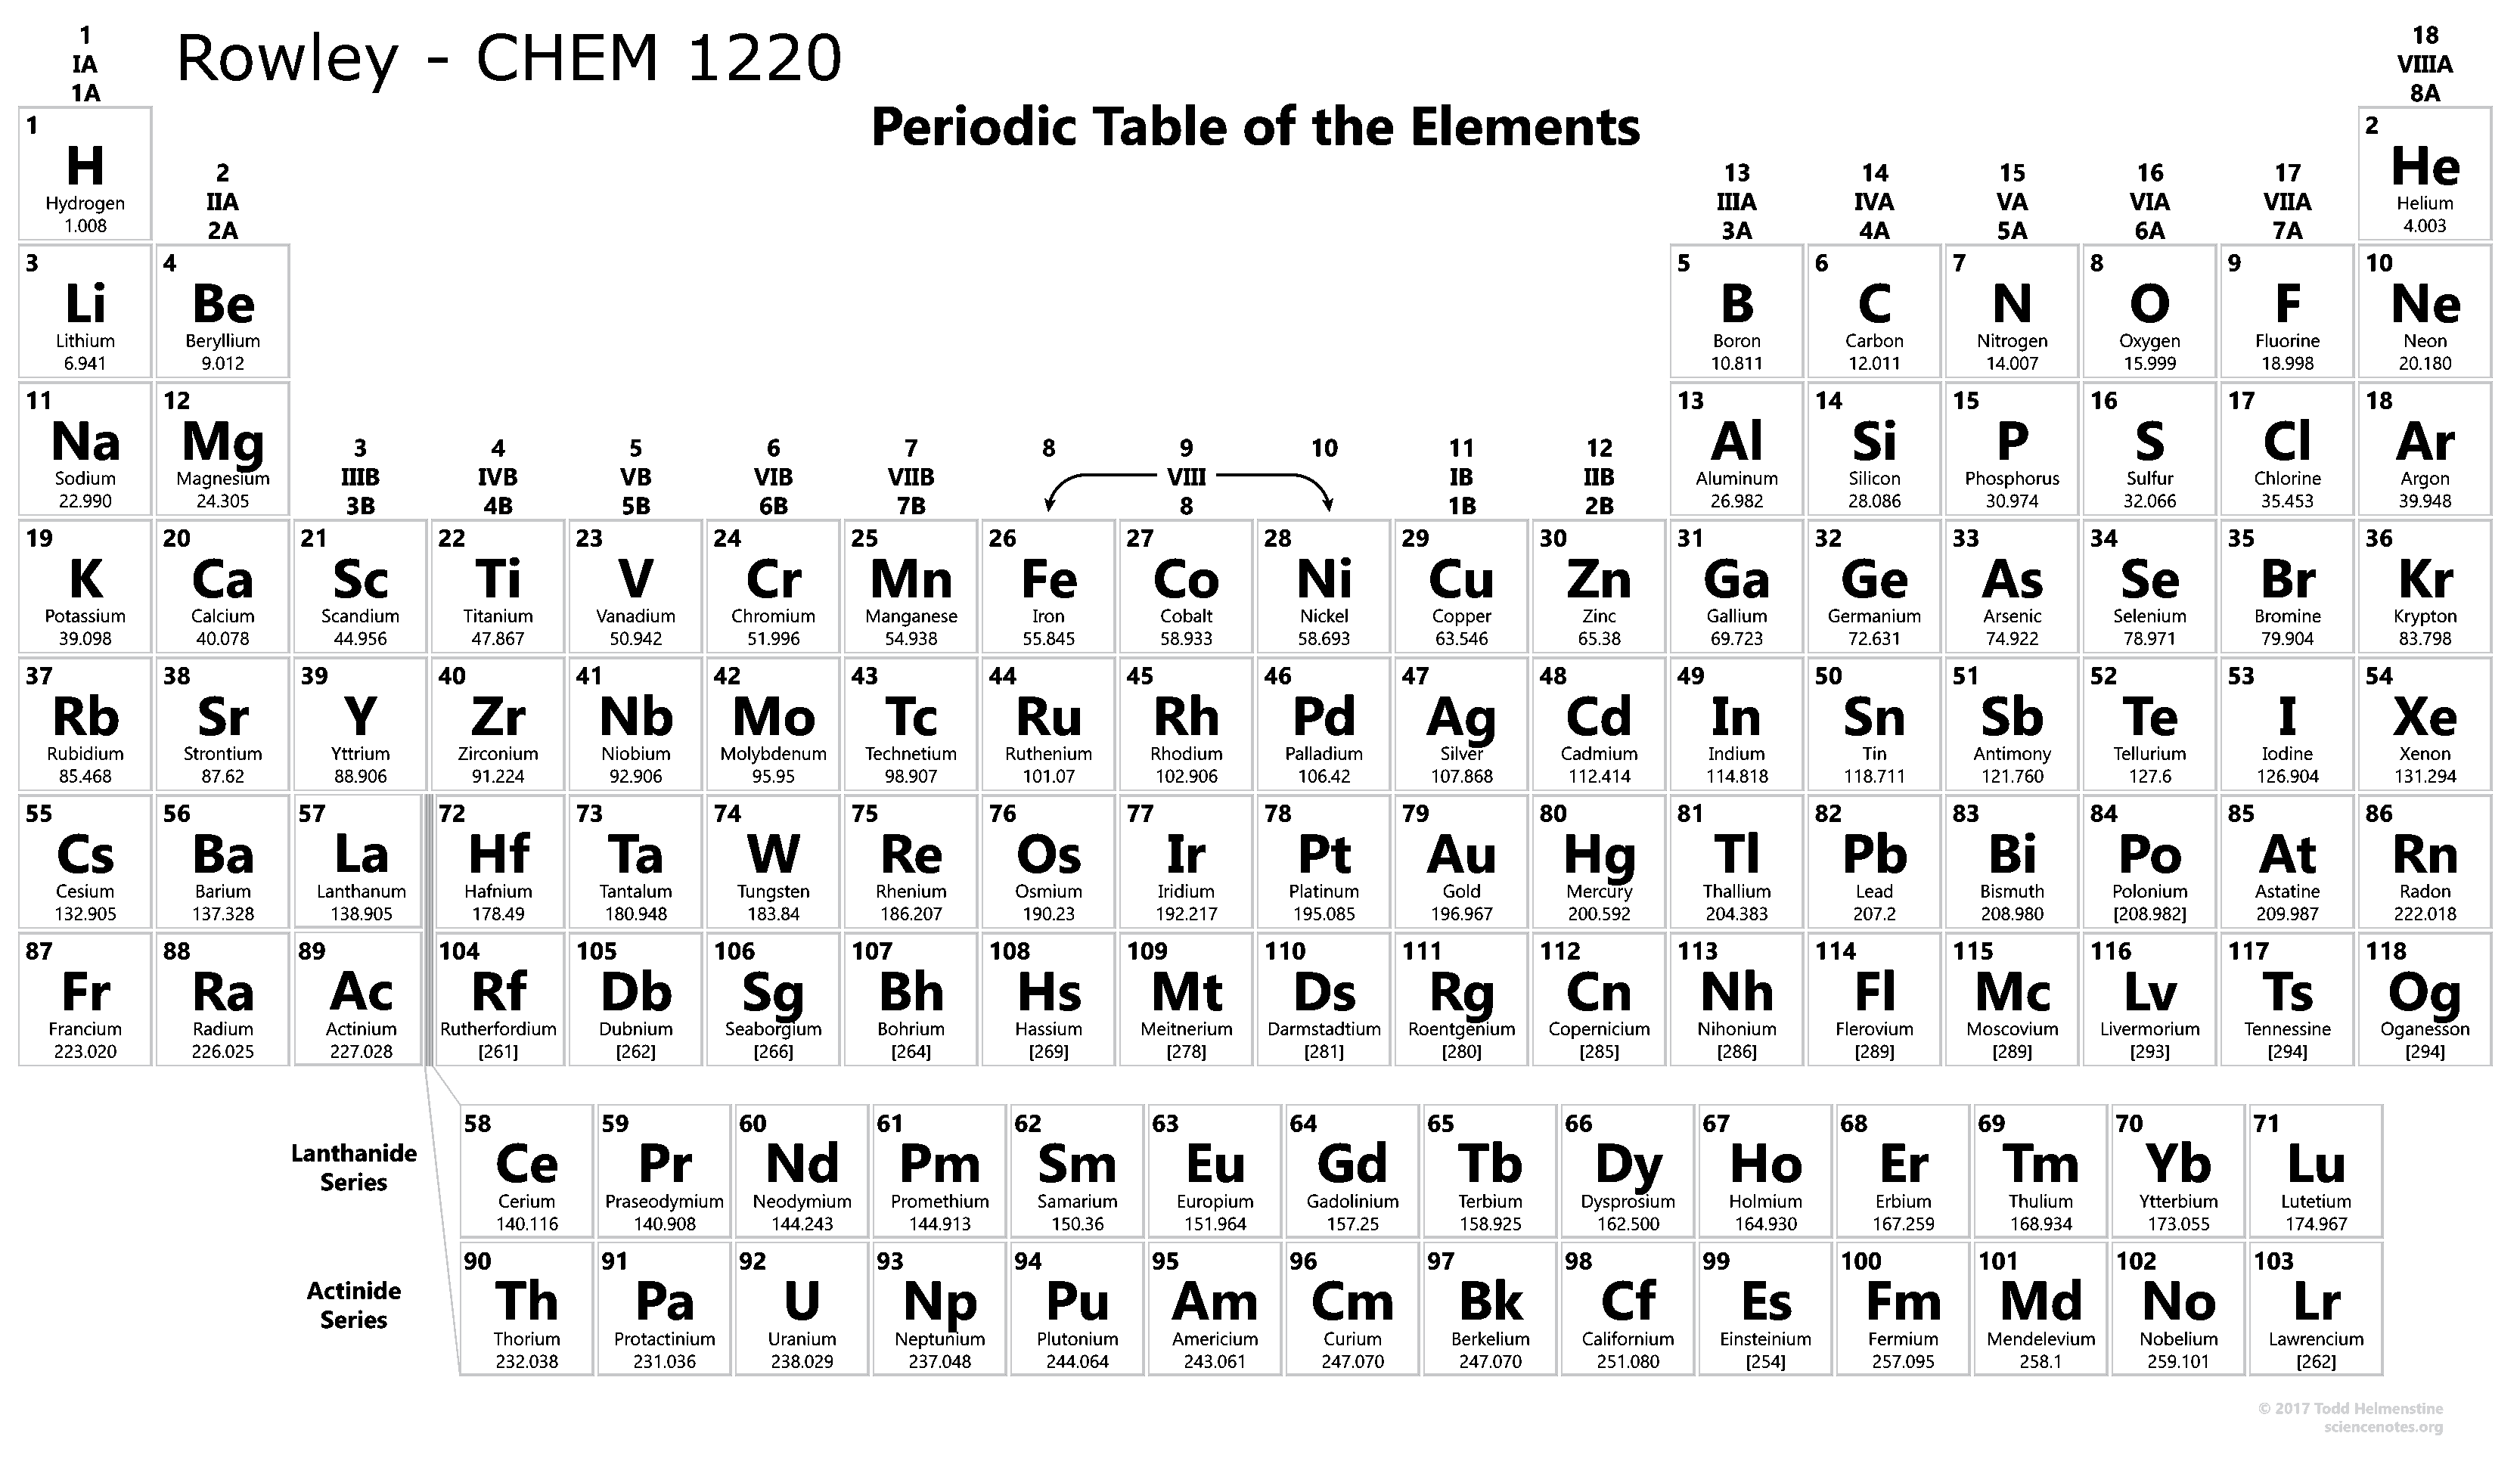
\includegraphics[width=1.3\textwidth, angle =90]{UpdatedTable.png}

	\restoregeometry

	
\end{document}